\documentclass{../../oss-classkick-exam}
\usetikzlibrary{decorations.pathmorphing,patterns}

\begin{document}
\genheader

\gentitle{4 \& 5}{MOMENTUM AND CENTER OF MASS}

\genmultidirections

\gengravity

\raggedcolumns
\begin{multicols*}{2}
  \begin{questions}
    \question A uniform rod of length $2\ell$ is bent, as shown in the figure
    below. What are the coordinates of the center of mass of the rod?
    \begin{center}
      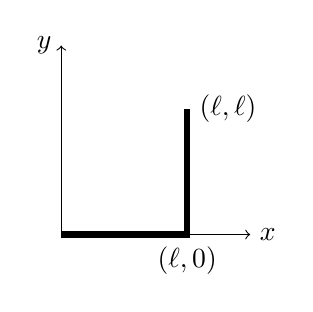
\begin{tikzpicture}[scale=.8]
        \draw[->](0,0)--(3,0) node[right]{$x$};
        \draw[->](0,0)--(0,3) node[left]{$y$};
        \draw[line width=.8mm](0,0)--(2,0) node[below]{$(\ell,0)$}
        --(2,2) node[right]{$(\ell,\ell)$};
      \end{tikzpicture}
    \end{center}
    \begin{choices}
      \choice $(\ell/4,3\ell/4)$
      \correctchoice $(3\ell/4,\ell/4)$
      \choice $(2\ell/3,\ell/3)$
      \choice $(2\ell/3,2\ell/3)$
      \choice $(\ell/2,\ell/3)$
    \end{choices}

    \question Two uniform spheres of mass $M$ and $4M$ are connected by a rod
    whose mass is negligible, and the distance between the centers of the
    spheres is $d$. The $4M$ sphere is then moved a distance of $d/3$ toward the
    smaller sphere. How far has the center of mass of the entire object moved?
    \begin{choices}
      \choice The center of mass has not moved, because both spheres still have
      their original masses.
      \choice $d/15$
      \choice $d/5$
      \correctchoice $4d/15$
      \choice $8d/15$
    \end{choices}
    
    \question A rubber ball of mass $m$ strikes a wall with a speed $\varv$ at
    an angle $\theta$ below the normal line and rebounds from the wall at the
    same speed and angle above the normal line as shown. The magnitude of the
    change in momentum of the ball is
    \begin{center}
      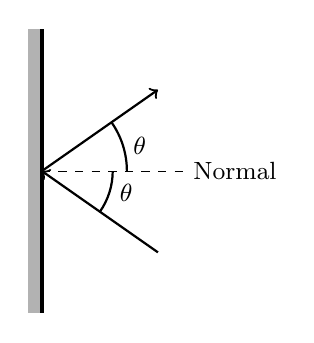
\begin{tikzpicture}[scale=.9]
        \fill[gray!60](-.2,2) rectangle(0,-2);
        \draw[very thick](0,-2)--(0,2);
        \draw[dashed](0,0)--(2,0) node[right]{\small Normal};
        \draw[->,rotate=35, thick](0,0)--(2,0) node[right]{$\varv$};
        \draw[<-,rotate=-35,thick](0,0)--(2,0) node[right]{$\varv$};
        \draw[thick](1,0)  arc(0:-35:1)  node[midway,right]{\small$\theta$};
        \draw[thick](1.2,0)arc(0: 35:1.2)node[midway,right]{\small$\theta$};
      \end{tikzpicture}
    \end{center}
    \begin{choices}
      \choice $m\varv$
      \choice $2m\varv$
      \choice $m\varv\cos\theta$
      \choice $2m\varv\cos\theta$
      \choice  zero
    \end{choices}
    
    \question Two blocks are connected by a compressed spring and rest on a
    frictionless surface. The blocks are released from rest and pushed apart
    by the compressed spring. If one mass is twice the mass of the other,
    which of the following is the same for both blocks?
    \begin{choices}
      \choice magnitude of momentum
      \choice acceleration
      \choice speed
      \choice kinetic energy
      \choice potential energy
    \end{choices}
    \vspace{.7in}
    
    \question A known net force $F$ acts on an unknown mass for a known time
    $\Delta t$. From this information, you could determine the
    \begin{choices}
      \choice change in kinetic energy of the object
      \choice change in velocity of the object
      \choice acceleration of the object
      \choice mass of the object
      \choice change in momentum of the object
    \end{choices}
    \columnbreak
    
%    \question Two billiard balls are rolling to the right on a table as shown.
%    The \SI{.4}{\kilo\gram} ball is moving faster than the \SI{.2}{\kilo\gram}
%    ball, so it catches up and strikes it from behind at a slight angle.
%    Immediately after the collision, the $y$-component of the
%    \SI{.4}{\kilo\gram} ball is \SI2{\metre\per\second} downward.
%    The $y$-component of the velocity of the \SI{.2}{\kilo\gram} ball must be
%    \begin{center}
%      \begin{tikzpicture}[scale=.5]
%        \draw[dashed,->](-3,0)--(4,0) node[right]{\small$x$};
%        \draw[dashed,->](0,-2)--(0,4) node[above]{\small$y$};
%        \draw(.3,.3) circle(.3) node[above]{\small\;\;\;\SI{.2}{\kilo\gram}};
%        \draw[->](.6,.3)--(1.6,.3) node[right]{\small$\varv_2$};
%        \draw(-2.3,-.5) circle(.5) node[below left]{\small\SI{.4}{kg}\;\;};
%        \draw[->](-1.8,-.5)--(-1,-.5) node[right]{\small$\varv_1$};
%      \end{tikzpicture}
%    \end{center}
%    \begin{choices}
%      \choice\SI1{\metre\per\second} upward
%      \choice\SI2{\metre\per\second} upward
%      \choice\SI1{\metre\per\second} downward
%      \choice\SI2{\metre\per\second} downward
%      \choice\SI4{\metre\per\second} upward
%    \end{choices}

    \question A small mass $m$ is moving with a speed $\varv$ toward a
    stationary mass $M$. The speed of the center of mass of the system is
    \begin{choices}
      \choice $\left(\dfrac m{m+M}\right)\varv$
      \choice $\left(\dfrac{m+M} m\right)\varv$
      \choice $\left(\dfrac mM\right)\varv$
      \choice $\left(1+\dfrac mM\right)\varv$
      \choice $\left(1+\dfrac M{3m}\right)\varv$
    \end{choices}

%    \question An object has a mass $4m$. The object explodes into three pieces
%    of mass $m$, $m$, and $2m$. The two pieces of mass $m$ move off at right
%    angles to each other with the same momentum $m\varv$, as shown below. The
%    speed of mass $2m$ after the explosion is
%    \begin{center}
%      \begin{tikzpicture}[scale=.4]
%        \draw[thick,dashed](-1.5,0)--(3,0);
%        \draw[thick,dashed](0,-1.5)--(0,3);
%        \draw[thick](0,0) circle(.5);
%        \fill[thick](-1.5,0) circle(.15) node[above]{\small $m$};
%        \fill[thick](0,-1.5) circle(.15) node[right]{\small $m$};
%          \draw[very thick,->](-1.5,0)--(-3,0)node[left]{\small$m\varv$};
%          \draw[very thick,->](0,-1.5)--(0,-3)node[below]{\small$m\varv$};
%      \end{tikzpicture}
%    \end{center}
%    \vspace{-.2in}
%    \begin{choices}
%      \choice $2\varv$
%      \choice $\sqrt 2\varv$
%      \choice $\dfrac{\sqrt 2}2\varv$
%      \choice $\dfrac{\sqrt 2}3\varv$
%      \choice $\dfrac{\sqrt 3}2\varv$
%    \end{choices}

    \uplevel{
      \textbf{Questions \ref{cm1}--\ref{cm2}}\\
      A projectile is launched at an angle to the level ground as shown. At the
      top of the trajectory at point $P$, the projectile explodes into two
      pieces of mass $2m$ and $m$.
      \cpic{.22}{exploding-projectile}
    }

    \question Which of the following arrows best represents the direction of the
    velocity of the center of mass of the projectile at point $P$ after the
    explosion?
    \label{cm1}
    \begin{choices}
      \choice{\huge$\leftarrow$}
      \choice{\huge$\swarrow$}
      \choice{\huge$\searrow$}
      \choice{\huge$\rightarrow$}
      \choice{\huge$\nearrow$}
    \end{choices}
    
    \question Which of the following statements is true of the center of mass
    of the projectile after the explosion?
    \label{cm2}
    \begin{choices}
      \choice The center of mass will continue on a parabolic path and land on
      the ground at the place where it would have landed had it not exploded.
      \choice The center of mass will alter its parabolic path and land on the
      ground farther from where it would have landed had it not exploded.
      \choice The center of mass will alter its parabolic path and land on the
      ground at a shorter distance than it would have landed had it not
      exploded.
      \choice The center of mass will fall straight downward from the point of
      explosion.
      \choice The center of mass will travel straight upward from the point of
      explosion.
    \end{choices}
    \vspace{.7in}
    
%    \uplevel{\textbf{Questions \ref{bfa1}--\ref{bfa2}}\\
%      Two balls are on a horizontal billiard table. A \SI1{\kilo\gram}
%      billiard ball moves downward along the $y$-axis with
%      a speed of \SI{16}{\metre\per\second} toward a \SI2{\kilo\gram} ball
%      that is at rest. The balls collide at an angle, and move along the lines
%      shown. After the collision, the \SI1{\kilo\gram} ball moves at
%      \SI9{\metre\per\second} along the $+x$-axis. The table below shows the
%      $x$ and $y$ components of the momentum in
%      \si{\kilo\gram\metre\per\second} of the two balls before and after the
%      collision.
%      \begin{center}
%        \begin{tabular}{lcccc}
%          \hline
%          & $p_{1x}$ & $p_{1y}$ & $p_{2x}$ & $p_{2y}$ \\ \hline
%          \textbf{Before Collision} & 0    & $-16$ &   0  & 0     \\ \hline
%          \textbf{After Collision}  & $+9$ & 0     & $-9$ & $-16$ \\ \hline 
%        \end{tabular}
%      \end{center}
%    }
%
%    \question Which of the following statements is true?
%    \begin{choices}    
%      \choice Momentum is conserved only in the $x$-direction in this collision.
%      \choice Momentum is conserved only in the $y$-direction in this collision.
%      \choice Momentum is conserved in both the $x$- and $y$-directions in this
%      collision
%      \choice The momentum of the 1 kg ball increases after the collision.
%      \choice The momentum of the 2 kg ball decreases after the collision.
%    \end{choices}
%    \label{bfa1}
%    
%    \question What is the speed of the \SI2{\kilo\gram} ball after the
%    collision?
%    \begin{choices}
%      \choice\SI{16}{\metre\per\second}
%      \choice\SI{9.2}{\metre\per\second}
%      \choice\SI{7.5}{\metre\per\second}
%      \choice\SI{6.}{\metre\per\second}
%      \choice\SI{5.}{\metre\per\second}
%    \end{choices}
%    \label{bfa2}
    
%    \uplevel{
%      \textbf{Questions \ref{3masses1}--\ref{3masses2}}\\
%      Three identical masses can slide freely on a horizontal surface as shown.
%      The first mass moves with a speed of \SI{3.}{\metre\per\second} toward
%      the second and third masses, which are initially at rest. The first and
%      second mass collide elastically, and then the second and third masses
%      collide inelastically.
%      \begin{center}
%        \begin{tikzpicture}
%          \fill[gray!50](0,0) rectangle(7,-.2);
%          \draw[thick](0,0)--(7,0);
%          \draw[thick](.8,0) rectangle(1.8,1);
%          \draw[thick](2.5,0) rectangle(3.5,1);
%          \draw[thick](5,0) rectangle(6,1);
%          \draw[very thick,->](5,.5)--(4,.5) node[midway,above]{\SI{3}{m/s}};
%        \end{tikzpicture}
%      \end{center}
%    }
%
%    \question The speed of the second mass after the collision is
%    \label{3masses1}
%    \begin{choices}
%      \choice zero
%      \choice\SI{1.5}{\metre\per\second}
%      \choice\SI{3.}{\metre\per\second}
%      \choice\SI{6.}{\metre\per\second}
%      \choice\SI{9.}{\metre\per\second}
%    \end{choices}
%
%  \question The speed of the second and third masses after they collide
%    inelastically is
%    \label{3masses2}
%    \begin{choices}
%      \choice zero
%      \choice\SI{1.5}{\metre\per\second}
%      \choice\SI{3.}{\metre\per\second}
%      \choice\SI{6.}{\metre\per\second}
%      \choice\SI{9.}{\metre\per\second}
%    \end{choices}

    \question A mass traveling in the $+x$ direction collides with a mass at
    rest. Which of the following statements is true?
    \begin{choices}
      \choice After the collision, the two masses will move with parallel
      velocities
      \choice After the collision, the masses will move with anti-parallel
      velocities
      \choice After the collision, the masses will both move along the $x$-axis
      \choice After the collision, the $y$-components of the velocities of the
      two particles will sum to zero.
      \choice None of the above
    \end{choices}
    \columnbreak
    
    \question A \SI{1000}{\kilo\gram} (empty mass) railroad car is rolling
    without friction on a horizontal track at a speed of
    \SI{2.}{\metre\per\second}. Sand is poured into the open top of the car for
    the time interval from $t=0$ to $t=\SI{4.}\second$. The mass of the sand
    poured into the car as a function of time is $m(t)=60t^2$. The velocity of
    the car at a time of \SI{4.}{\second} is most nearly
    \cpic{.25}{railroad-car-sand}
    \begin{choices}
      \choice\SI1{\metre\per\second}
      \choice\SI2{\metre\per\second}
      \choice\SI3{\metre\per\second}
      \choice\SI4{\metre\per\second}
      \choice\SI5{\metre\per\second}
    \end{choices}
    
    \uplevel{
      \textbf{Questions \ref{ramps1}--\ref{ramps2}}\\
      A small block of mass $m$ slides on a horizontal frictionless surface
      toward a ramp of mass $3m$ which is also free to move on the surface. The
      small block slides up to a height $h$ on the ramp with no friction
      (Figure I), then they move together (Figure II), and the small block
      slides back down the ramp to the horizontal surface (Figure III). Both
      the block and the ramp continue to slide on the horizontal surface after
      they separate.
      \cpic{.27}{Figs123}
    }

    \question Which of the following is true regarding the conservation laws
    throughout this process?
    \label{ramps1}
    \begin{choices}
      \choice Kinetic energy is conserved from I to II.
      \choice Momentum is conserved from I to III.
      \choice Kinetic energy is conserved from II to III.
      \choice Potential energy is conserved from I to II.
      \choice Potential energy is conserved from II to III.
    \end{choices}
    \vspace{.7in}
    
    \question Which of the following is a true statement regarding Figure III?
    \label{ramps2}
    \begin{choices}
      \choice The small block is moving to the left and the ramp is moving to
      the right.
      \choice The small block is moving to the right and the ramp is moving
      to the left.
      \choice The small block is moving to the right and the ramp is moving
      to the right.
      \choice The small block is moving to the left and the ramp is moving to
      the left.
      \choice The small block and the large block are moving with the same
      velocity.
    \end{choices}
    \vspace{.7in}
    
%    \uplevel{
%      \textbf{Questions \ref{remote1}--\ref{remote2}}
%
%      A remote controlled stunt car of mass \SI{800}{\kilo\gram} initially
%      moving at \SI{10}{\metre\per\second} is crashed into a rail car of mass
%      $m$ that is initially at rest. The cars stick together, and the speed
%      $\varv$ of both cars after the collision is given by
%      $\varv=\dfrac6{t+1}$.
%    }
%
%    \question By considering the fact that the crash occurs at time $t=0$,
%    determine the mass $m$ of the rail car.
%    \label{remote1}
%    \begin{choices}
%      \choice\SI{288}{\kilo\gram}
%      \choice\SI{445}{\kilo\gram}
%      \choice\SI{533}{\kilo\gram}
%      \choice\SI{698}{\kilo\gram}
%      \choice\SI{800}{\kilo\gram}
%    \end{choices}
%    
%    \question The magnitude of the resisting force acting on the cars as a
%    function of time after the collision is
%    \label{remote2}
%    \begin{choices}
%      \choice $\dfrac{6m}{t+1}$
%      \choice $6m(t+1)$
%      \choice $6m(t+1)^2$
%      \choice $\dfrac{6m}{(t+1)^2}$
%      \choice $\dfrac{m(t+1)^2}6$
%    \end{choices}
    \columnbreak
    
    \question A moving object is changing its momentum during a time interval.
    If a graph of momentum vs.\ time is plotted, the net force acting on the
    mass at any time can be determined by finding the
    \begin{choices}
      \choice slope of line tangent to the graph at that time
      \choice area under the graph
      \choice $y$-intercept of the graph
      \choice $x$-intercept of the graph
      \choice change in slope of the graph from beginning to end
    \end{choices}
    \vspace{.7in}
    
    \question A mass $m_1$ initially moving at speed $\varv_0$ collides with and
    sticks to a spring attached to a second, initially stationary mass $m_2$.
    The two masses continue to move to the right on a frictionless surface as
    the length of the spring oscillates. At the instant that the spring is
    maximally extended, the velocity of the first mass is
    \begin{center}
      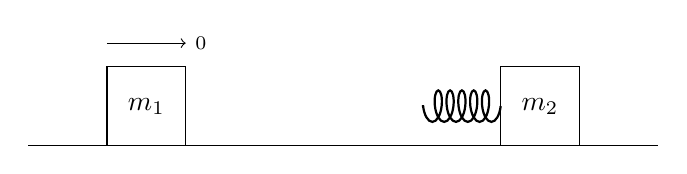
\begin{tikzpicture}
        \draw[->](1,1.3)--(2,1.3) node[pos=1,right]{$\varv_0$};
        \draw(0,0)--(8,0);
        \draw(1,0) rectangle (2,1) node[midway]{$m_1$};
        \draw(6,0) rectangle (7,1) node[midway]{$m_2$};
        \draw[thick,
          decoration={aspect=.4,segment length=1.5mm, amplitude=2mm,coil},
          decorate] (6,.5)--(5,.5);
      \end{tikzpicture}
    \end{center}
    \begin{choices}
      \choice $\varv_0$
      \choice $m_1^2\varv_0/(m_1+m_2)^2$
      \choice $m_2\varv_0/m_1$
      \choice $m_1\varv_0/m_2$
      \choice $m_1\varv_0/(m_1+m_2)$
    \end{choices}
  \end{questions}
\end{multicols*}
\newpage


\genfreetitle{4 \& 5}{MOMENTUM, IMPULSE, COLLISIONS, AND CENTER OF MASS}{3}

\genfreedirections

% THIS QUESTION CAME FROM ONE OF THE REFERENCE BOOKS THAT I USED FOR PREPARING
% FOR AP PHYSICS C. IT'S NOT A BAD QUESTION, BUT IMMENSELY TEDIOUS AND DOES
% NOT ADD ANYTHING MEANINGFUL TO THE LEARNING PROCESS. IT CAN BE RE-USED FOR
% OTHER COURSES LATER.
  
%  \question A projectile is fired from the edge of a cliff \SI{100}{\metre}
%  high with an initial speed of \SI{60}{\metre\per\second} at an angle of
%  elevation of \ang{45}.
%  \begin{parts}
%    \part Write equation for $x(t)$, $y(t)$, $\varv_x(t)$ and $\varv_y(t)$.
%    Choose the origin of your coordinate system at the particle's original
%    location.
%
%    \part Calculate the location and velocity of the particle at time
%    $t=\SI5\second$.
%    
%    \uplevel{Suppose the projectile experiences an internal explosion at time
%      $t=\SI4\second$ with an internal force purely in the $y$-direction,
%      causing it to break into a \SI2{\kilo\gram} and a \SI1{\kilo\gram}
%      fragment.}
%    
%    \part If the \SI2{\kilo\gram} fragment is \SI{77}{\metre} above the height
%    of the cliff at $t=\SI5\second$, what is the $y$-coordinate of the position
%    of the \SI1{\kilo\gram} piece?
%    
%    \part If the speed of the \SI2{\kilo\gram} fragment is
%    \SI{46}{\metre\per\second} and the fragment is falling at $t=\SI5\second$,
%    what is the $y$-component of the velocity of the \SI1{\kilo\gram} fragment?
%  \end{parts}
%  \newpage

% TAKEN FROM THE 2015 AP PHYSICS C MECHANICS EXAM FREE-RESPONSE QUESTION 2
\cpic{.5}{dart}
  \begin{questions}    
  \question A small dart of mass \SI{.020}{\kilo\gram} is launched at an angle
  of \ang{30} above the horizontal with an initial speed of
  \SI{10}{\meter\per\second}. At the moment it reaches the highest point in its
  path and is moving horizontally, it collides with and sticks to a wooden
  block of mass \SI{.10}{\kilo\gram} that is suspended at the end of a massless
  string. The center of mass of the block is \SI{1.2}{\metre} below the pivot
  point of the string. The block and dart then swing up until the string makes
  an angle $\theta$ with the vertical, as shown above. Air resistance is
  negligible.
  \begin{parts}
    \part Determine the speed of the dart just before it strikes the block.
    
    \part Calculate the horizontal distance $d$ between the launching point of
    the dart and a point on the floor directly below the block.
    
    \part Calculate the speed of the block just after the dart strikes.
    
    \part Calculate the angle $\theta$ through which the dart and block on the
    string will rise before coming momentarily to rest.
    
    \part The block then continues to swing as a simple pendulum. Calculate the
    time between when the dart collides with the block and when the block first
    returns to its original position.

    \part In a second experiment, a dart with more mass is launched at the same
    speed and angle. The dart collides with and sticks to the same wooden block.
    \begin{subparts}
      \subpart Would the angle $\theta$ that the dart and block swing to
      increase, decrease, or stay the same? Justify your answer.

      \vspace{.1in}
      \underline{\hspace{.3in}} Increase\hspace{.6in}
      \underline{\hspace{.3in}} Decrease\hspace{.6in}
      \underline{\hspace{.3in}} Stay the same

      \subpart Would the period of oscillation after the collision increase,
      decrease, or stay the same? Justify your answer.

      \vspace{.1in}
      \underline{\hspace{.3in}} Increase\hspace{.6in}
      \underline{\hspace{.3in}} Decrease\hspace{.6in}
      \underline{\hspace{.3in}} Stay the same
    \end{subparts}
  \end{parts}
  \newpage
  
  % TAKEN FROM THE 2002 AP PHYSICS C EXAM FREE-RESPONSE QUESTION MECH 1
  \question A crash test car of mass \SI{1000}{\kilo\gram} moving at constant
  speed of \SI{12}{\metre\per\second} collides completely inelastically with an
  object of mass $M$ at time $t=0$. The object was initially at rest. The speed
  $\varv$ in m/s of the car-object system after the collision is given as a
  function of time $t$ in seconds by the expression
  \begin{displaymath}
    \varv=\frac8{1 + 5t}
  \end{displaymath}
  \begin{parts}
    \part Calculate the mass $M$ of the object.
    
    \part Assuming an initial position of $x=0$, determine an expression for
    the position of the car-object system after the collision as a function of
    time $t$.
    
    \part Determine an expression for the resisting force on the car-object
    system after the collision as a function of time $t$.

    \part Determine the impulse delivered to the car-object system from $t=0$
    to $t=\SI{2.}\second$.
  \end{parts}
  \newpage
  
%  \uplevel{
%    \centering
%    \begin{tikzpicture}[scale=1.2]
%      \draw[thick,fill=gray!70](0,0) rectangle(-1,1) node[midway]{$m$};
%      \draw[thick,fill=gray!70](-3,0) rectangle(-4,1) node[midway]{$m$};
%      \draw[
%        thick,
%        decoration={aspect=.3,segment length=2mm, amplitude=2mm, coil},
%        decorate] (-1,.5)--(-3,.5);
%      \draw[very thick](-6,0)--(0,0)--(0,2);
%    \end{tikzpicture}
%  }
%  
%  \question Two masses are connected by a spring (spring constant $k$) resting
%  on a frictionless horizontal surface as shown. The right mass is initially in
%  contact with a wall. A brief blow to the left block leaves it with an initial
%  velocity $\varv_0$ to the right.
%  \begin{parts}
%    \part What is the maximum compression of the spring as the left block moves
%    to the right?
%    \label{maxcomp}
%    
%    \uplevel{After the spring is maximally compressed, it eventually moves to
%      the left, away from wall. As it moves away from the wall, it continues
%      oscillating.
%    }
%    
%    \part What is the net momentum of the two masses after they leave the wall?
%    
%    \part What is the total mechanical energy of the oscillating spring system?
%    
%    \part What is the relative velocity of the two masses when the spring is
%    maximally compressed?
%    
%    \part What is the maximum compression of the spring after the two masses
%    have left the wall? Compare the compression to the maximum compression
%    calculated in part (\ref{maxcomp}) and explain any similarities and
%    differences.
%  \end{parts}
%  \newpage

  \uplevel{
    \cpic{.25}{projectile}
  }
  \question A projectile is fired horizontally from a launching device, exiting
  with a speed $\varv_x$. While the projectile is in the launching device, the
  impulse imparted to it is $J$, and the average force on it is $F_\text{avg}$.
  Assume the force becomes zero just as the projectile reaches the end of the
  launching device. Express your answers to parts (a) and (b) in
  terms of $\varv_x$, $J$, $F_\text{avg}$, and fundamental constants, as
  appropriate.
  \begin{parts}
    \part Determine an expression for the time required for the projectile to
    travel the length of the launching device.
    
    \part Determine an expression for the mass of the projectile.
    
    \uplevel{The projectile is fired horizontally into a block of wood that is
      clamped to a tabletop so that it cannot move. The projectile travels a
      distance $d$ into the block before it stops. Express all algebraic
      answers to the following in terms of $d$ and the given quantities
      previously indicated, as appropriate.}

    \part Derive an expression for the work done in stopping the projectile.
    
    \part Derive an expression for the average force $F_b$ exerted on the
    projectile as it comes to rest in the block.
    \label{this}

    \uplevel{Now a new projectile and block are used, identical to the first
      ones, but the block is not clamped to the table. The projectile is again
      fired into the block of wood and travels a new distance $d_n$ into the
      block while the block slides across the table a short distance $D$.
      Assume the following: the projectile enters the block with speed
      $\varv_x$, the average force $F_b$ between the projectile and the block
      has the same value as determined in part (\ref{this}), the average force
      of friction between the table and the block is $f_T$, and the collision is
      instantaneous so the frictional force is negligible during the collision.
    }

    \part Derive an expression for $d_n$ in terms of $d$, $D$, $f_T$, and $F_b$,
    as appropriate.
    
    \part Derive an expression for $d_n$ in terms of $d$, the mass $m$ of the
    projectile, and the mass $M$ of the block.
  \end{parts}
\end{questions}
\end{document}
